\chapter{Appendix}\label{ch:appendix}
\textit{In this chapter additional data concerning the analyses led on the dataset are reported.}
\vspace{0.25cm}
\par\fancybreak{$***$}\par
\vspace{0.35cm}

\begin{figure}[h]
 \centering
     \begin{subfigure}[b]{0.24\textwidth}
         \centering
         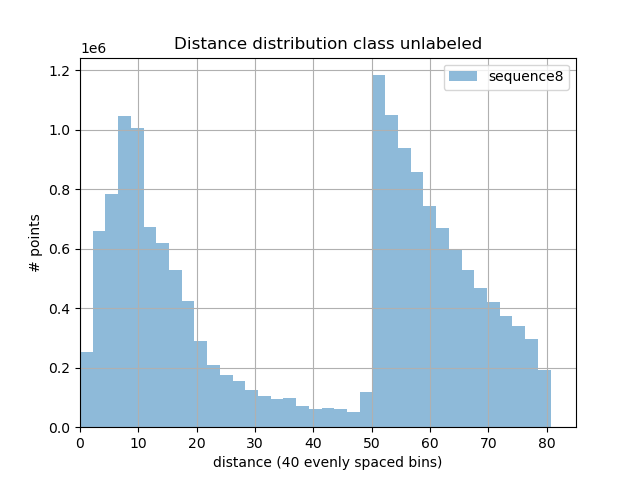
\includegraphics[width=\textwidth]{Figures/Chapter4/dist-height/dist/test/class0.png}
     \end{subfigure}
     \hfill
     \begin{subfigure}[b]{0.24\textwidth}
         \centering
         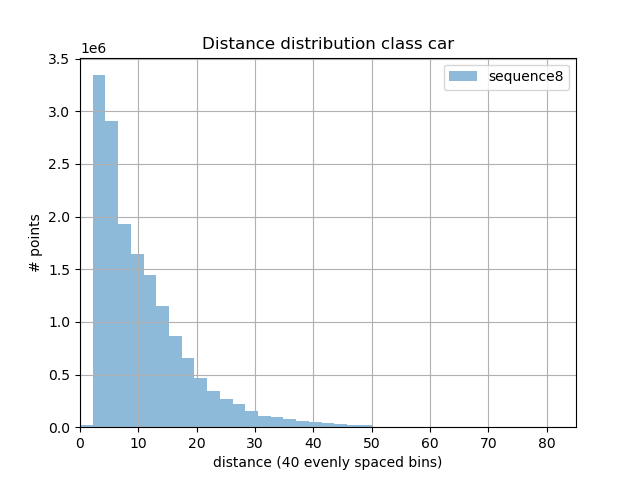
\includegraphics[width=\textwidth]{Figures/Chapter4/dist-height/dist/test/class1.png}
     \end{subfigure}
     \begin{subfigure}[b]{0.24\textwidth}
         \centering
         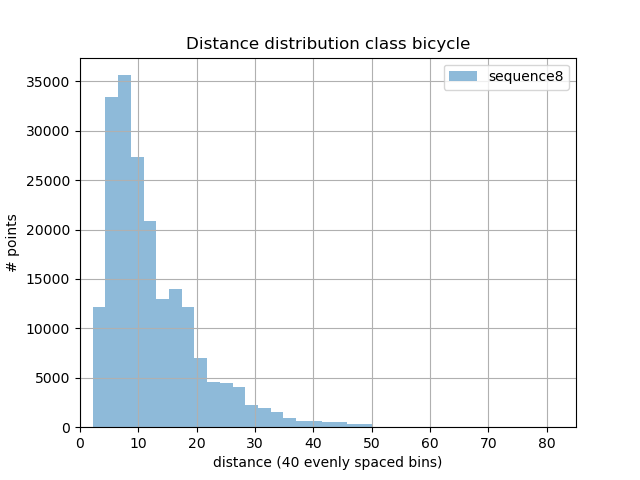
\includegraphics[width=\textwidth]{Figures/Chapter4/dist-height/dist/test/class2.png}
     \end{subfigure}
     \hfill
     \begin{subfigure}[b]{0.24\textwidth}
         \centering
         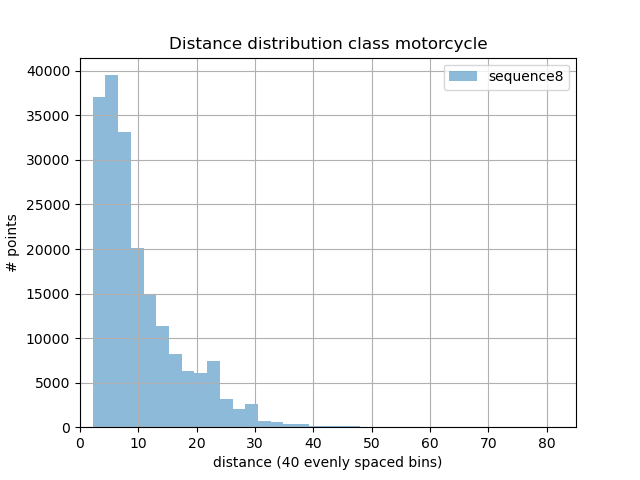
\includegraphics[width=\textwidth]{Figures/Chapter4/dist-height/dist/test/class3.png}
     \end{subfigure}
     \begin{subfigure}[b]{0.24\textwidth}
         \centering
         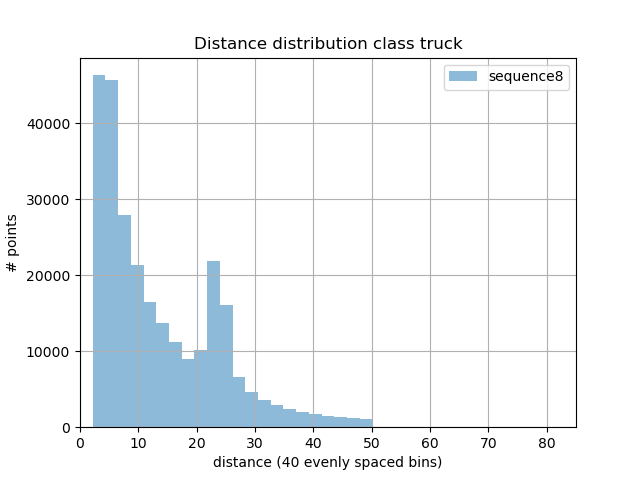
\includegraphics[width=\textwidth]{Figures/Chapter4/dist-height/dist/test/class4.png}
     \end{subfigure}
     \hfill
     \begin{subfigure}[b]{0.24\textwidth}
         \centering
         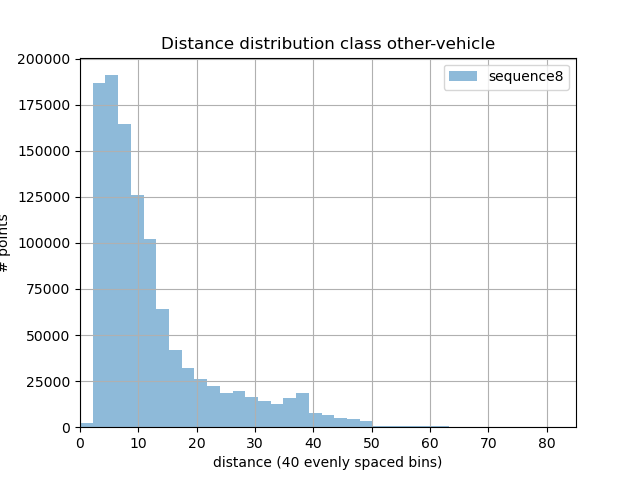
\includegraphics[width=\textwidth]{Figures/Chapter4/dist-height/dist/test/class5.png}
     \end{subfigure}
     \begin{subfigure}[b]{0.24\textwidth}
         \centering
         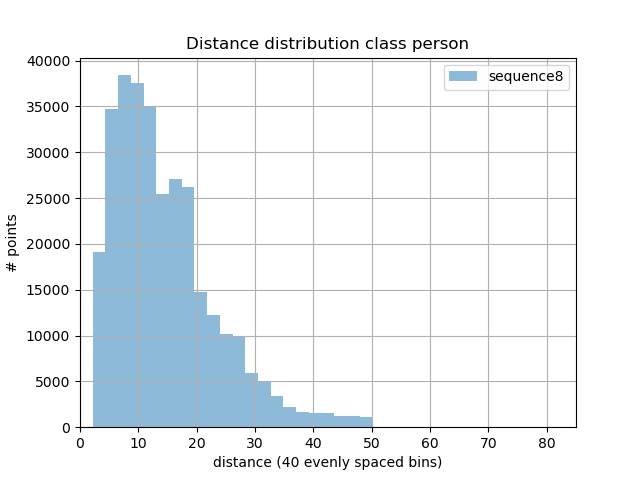
\includegraphics[width=\textwidth]{Figures/Chapter4/dist-height/dist/test/class6.png}
     \end{subfigure}
     \hfill
     \begin{subfigure}[b]{0.24\textwidth}
         \centering
         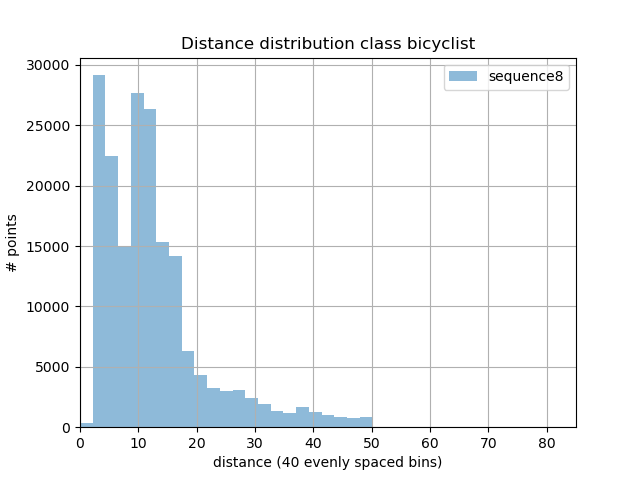
\includegraphics[width=\textwidth]{Figures/Chapter4/dist-height/dist/test/class7.png}
     \end{subfigure}
     \begin{subfigure}[b]{0.24\textwidth}
         \centering
         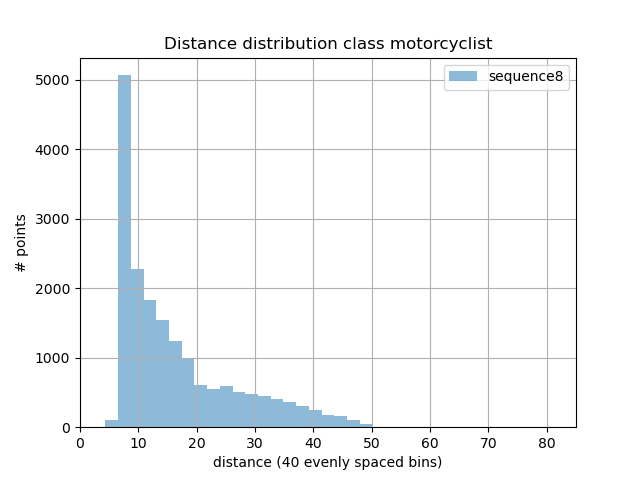
\includegraphics[width=\textwidth]{Figures/Chapter4/dist-height/dist/test/class8.png}
     \end{subfigure}
     \hfill
     \begin{subfigure}[b]{0.24\textwidth}
         \centering
         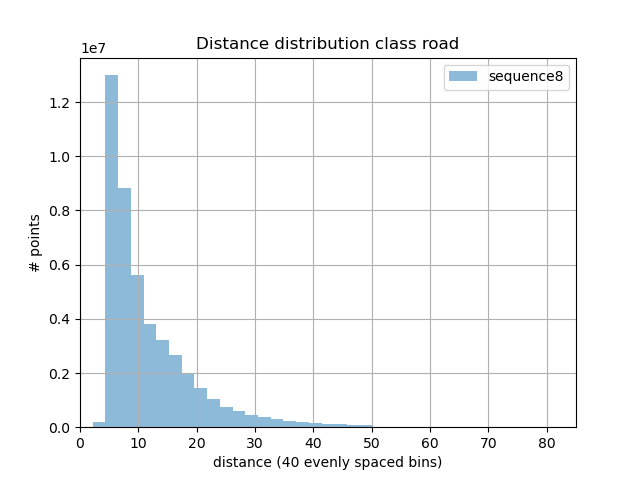
\includegraphics[width=\textwidth]{Figures/Chapter4/dist-height/dist/test/class9.png}
     \end{subfigure}
     \begin{subfigure}[b]{0.24\textwidth}
         \centering
         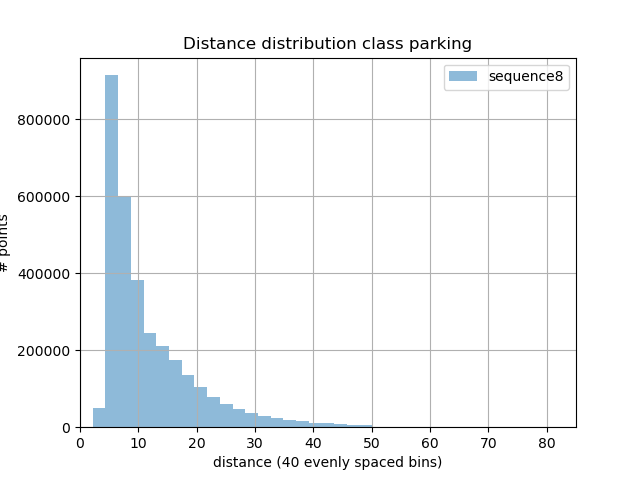
\includegraphics[width=\textwidth]{Figures/Chapter4/dist-height/dist/test/class10.png}
     \end{subfigure}
     \hfill
     \begin{subfigure}[b]{0.24\textwidth}
         \centering
         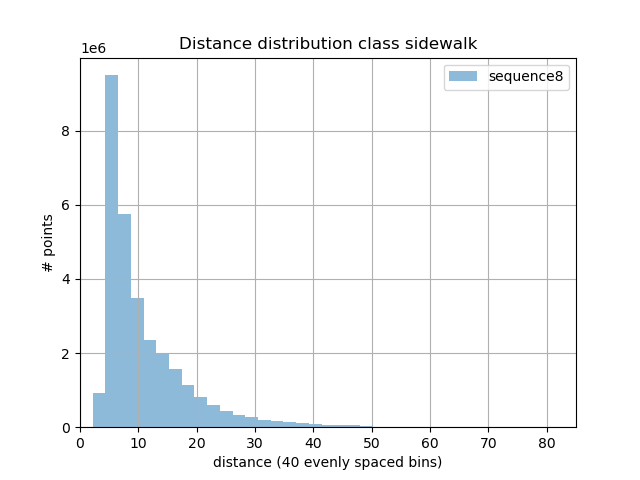
\includegraphics[width=\textwidth]{Figures/Chapter4/dist-height/dist/test/class11.png}
     \end{subfigure}
     \begin{subfigure}[b]{0.24\textwidth}
         \centering
         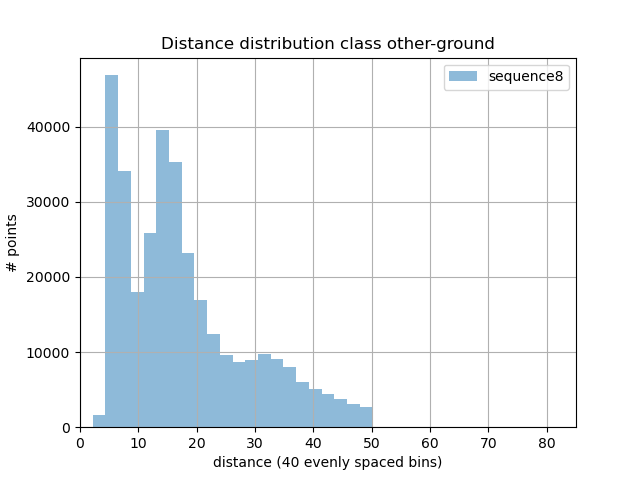
\includegraphics[width=\textwidth]{Figures/Chapter4/dist-height/dist/test/class12.png}
     \end{subfigure}
     \hfill
     \begin{subfigure}[b]{0.24\textwidth}
         \centering
         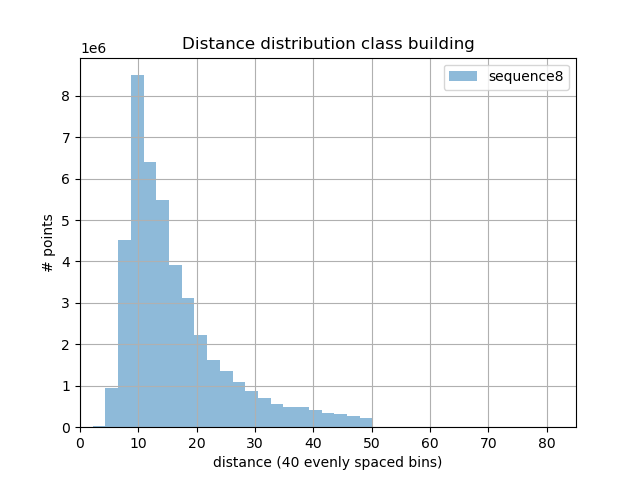
\includegraphics[width=\textwidth]{Figures/Chapter4/dist-height/dist/test/class13.png}
     \end{subfigure}
     \begin{subfigure}[b]{0.24\textwidth}
         \centering
         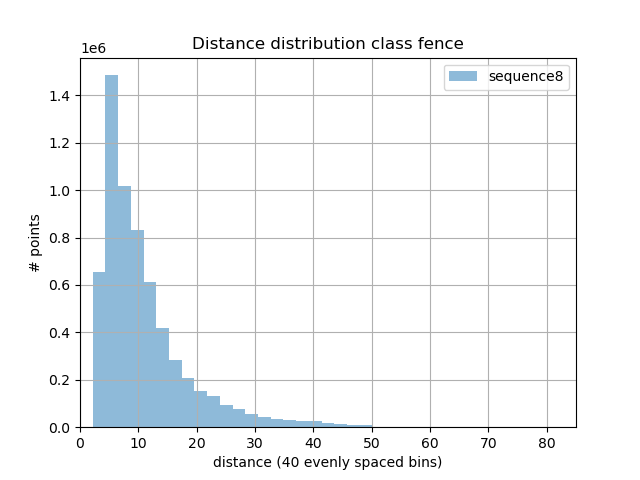
\includegraphics[width=\textwidth]{Figures/Chapter4/dist-height/dist/test/class14.png}
     \end{subfigure}
     \hfill
     \begin{subfigure}[b]{0.24\textwidth}
         \centering
         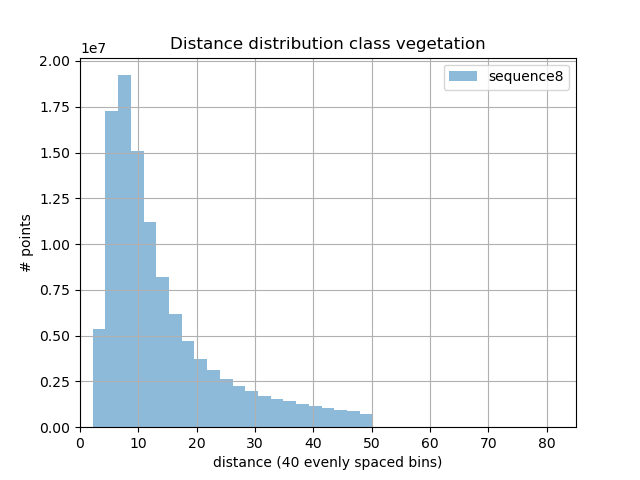
\includegraphics[width=\textwidth]{Figures/Chapter4/dist-height/dist/test/class15.png}
     \end{subfigure}
     \begin{subfigure}[b]{0.24\textwidth}
         \centering
         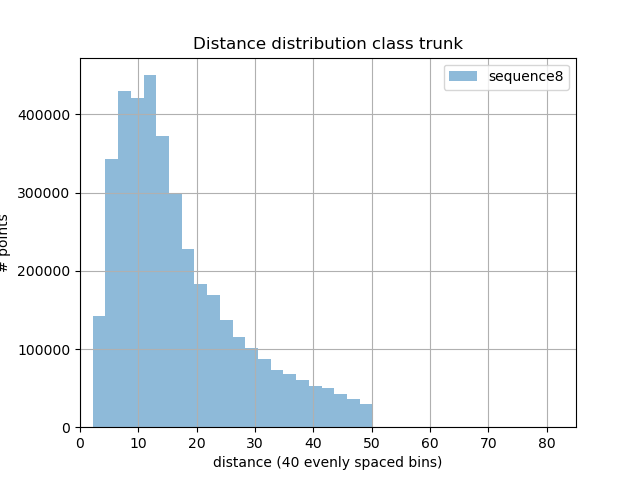
\includegraphics[width=\textwidth]{Figures/Chapter4/dist-height/dist/test/class16.png}
     \end{subfigure}
     \hfill
     \begin{subfigure}[b]{0.24\textwidth}
         \centering
         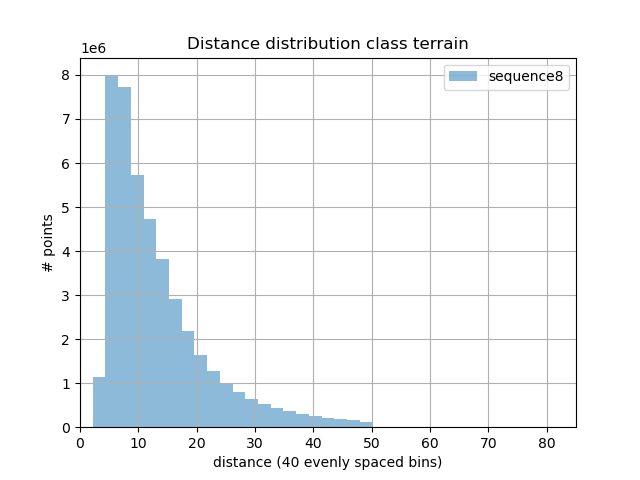
\includegraphics[width=\textwidth]{Figures/Chapter4/dist-height/dist/test/class17.png}
     \end{subfigure}
     \begin{subfigure}[b]{0.24\textwidth}
         \centering
         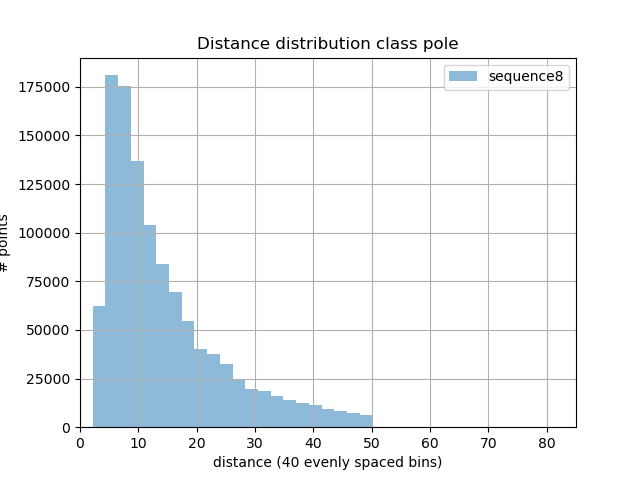
\includegraphics[width=\textwidth]{Figures/Chapter4/dist-height/dist/test/class18.png}
     \end{subfigure}
     \hfill
     \begin{subfigure}[b]{0.24\textwidth}
         \centering
         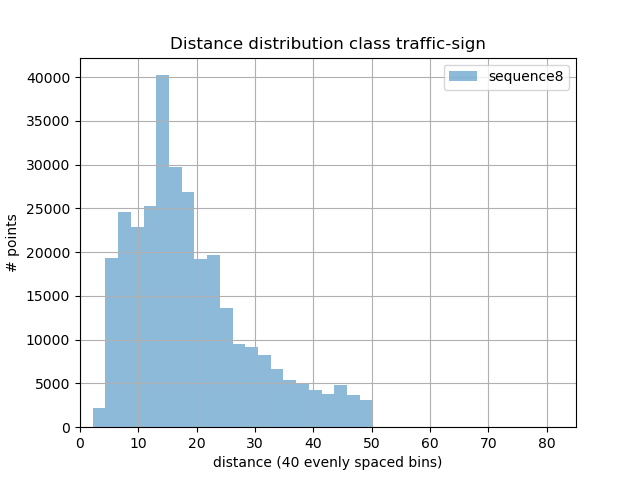
\includegraphics[width=\textwidth]{Figures/Chapter4/dist-height/dist/test/class19.png}
     \end{subfigure}
\caption{Example compuond figure.}        
\label{fig:distances}
\end{figure}